\section{Modell Parameter}
\label{Kapitel:Parameter}
Um eine realistische Simulation zu ermöglichen, ist es notwendig die verwendeten Modelle möglichst genau an Messdaten der realen Mörtel anzupassen. Dazu koe;nnen die materialabhae;ngigen Parameter in den Modellen variiert werden.\\
Für einige der Mörtel wurden die Parameter, die im verwendeten Modell \eqref{eq:modHB} vorkommen, schon in früheren Arbeiten bestimmt. \\
Einerseits wurden aber in der Zwischenzeit neue Mörtel entwickelt und andererseits ist es wünschenswert, ein Tool zur automatischen Bestimmung dieser Parameter zu haben das unabhängig von Drittanbietern in Form von Lizenzen und Support ist. \\
Dies wurde mithilfe einer Kombination aus \openfoam{} und der Programmiersprache Python umgesetzt.
%
\subsection{Messaufbau}
Die Messungen wurden von einem Hilti-internen Rheologen durchgeführt. Verwendet wurden zwei Messgeräte, ein Platte-Platte Rheometer und ein Kapillarrheometer.\\
Dabei wird in beiden Geräten das Fluid in eine einachsige, laminare Strömung versetzt, die es erlauben anhand einer Messgrösse die Viskosität abhängig von der Scherrate zu bestimmen.
%
\subsubsection{Platte-Platte Rheometer}
\label{Kapitel:Parameter:PlattePlatteRheo}
Das Platte-Platte Rheometer besteht aus zwei zylindrischen Platten, die so montiert sind dass zwischen ihnen ein schmaler, ebenfalls zylinderfoe;rmiger Spalt entsteht. \todo{Bild Rheometer}
Die Flüssigkeit wird in diesem Scherspalt platziert, der in radialer Richtung von einem Ring abgeschlossen werden kann. Beim Messvorgang wird die eine Platte fixiert, die andere mit einer vorgegebenen Geschwindigkeit $\Omega$ gedreht.
Dabei wird das benötigte Drehmoment gemessen, das für die Drehgeschwindigkeit aufgewendet werden muss.
\todo{Formeln Berechnung Viskositaet}

Das Platte-Platte Rheometer eignet sich ebenfalls dazu, zeitabhängige Effekte wie die Relaxationszeit eines viskoelastischen Fluids zu messen. 
Dazu wird die obere Platte nicht mit einer konstanten Geschwindigkeit bewegt, sondern mit einer schwingungsähnlichen Drehung auf die eine oder die andere Seite bewegt.
\todo{Schwingungs Modi}
%
\begin{todocontent}
    \1 Beschreibung Rheometer
    \1 Bilder von Messkurven
\end{todocontent}
%
\subsubsection{Kapillarrheometer}
Das Kapillarrheometer kann wie das Platte-Platte Rheometer zur Bestimmung der scherratenabhängigen Viskosität verwendet werden. Das Fluid wird dabei aber nicht gedreht, sondern durch eine zylinderfoe;rmige Kapillare gepresst. Als Messgroe;sse dient dabei der Druckunterschied.\\
Um dabei den durch das Mitmessen des Einlaufdruckverlustes (Bagley-Druck) gemachten systematischen Fehler zu korrigieren, wird meistens parallel zum eigentlichen Kapillarrheomter auch noch der Druckverlust in einer Nullblende gemessen, wie in Abbildung (x) dargestellt. \todo{Bild Kapillarrheometer}

Die Beziehung der Messgroe;sse $\Delta p_{\mbox{\tiny Mess}}$ zu der Schubspannung $\tau$ ist dabei wie folgt:
\begin{equation}
    \label{eq:KapRheoTau}
    \tau\left( R \right) = \frac{R \Delta p}{2L}
\end{equation}
wobei $\Delta p = \Delta p_{\mbox{\tiny Mess}} -\Delta p_{\mbox{\tiny Bagley}}$ der korrigierte Druckunterschied ist und $L$ und $R$ die Lae;nge respektive der Radius der Kapillare sind.

Fue;r die Berechnung der in der Kapillare auftretenden Scherrate kann die Beziehung
\begin{equation}
    \label{eq:KapRheoScherrate}
    \gammap = \frac{4 \dot{V}}{\pi R^3}\left( \frac{3+n}{4} \right) \mbox{ mit } n=\frac{d \ln \dot{V}}{d\ln\tau}
\end{equation}
verwendet werden.

Mit Hilfe von \eqref{eq:KapRheoTau} und \eqref{eq:KapRheoScherrate} lae;sst sich die Fliesskurve 
\begin{equation}
    \eta(\gammap) = \frac{\tau}{\gammap}
\end{equation}
mit dem gemessenen Druckunterschied bei einem vorgegebenen Volumenstrom bestimmen.
%
\begin{todocontent}
    \1 Bilder von Messkurven
\end{todocontent}
%
\subsection{Korrektursimulation}
\label{Kapitel:Korrektursimulation}
Die in Kapitel \ref{Kapitel:Parameter:PlattePlatteRheo} beschriebenen Rheometer messen das für eine vorgegebene Geschwindigkeit benötigte Drehmoment. Daraus kann die Viskosität des Fluides berechnet werden.\\
Um zu verhindern, dass der Mörtel während der Messung in radialer Richtung aus dem Gerae;t fliesst, wurde um den Scherspalt ein Ring montiert. Dadurch wird zwar ein Herausfliessen verhindert, gleichzeitig wird aber die Messung verfälscht. Der Ring ist eine zusätzliche Wand an der das Fluid entlangströmen muss, was in ein erhöhtes Drehmoment und damit eine hoe;here gemessene Viskositae;t zur Folge hat.

Um trotzdem eine zuverlässige Bestimmung der Modell-Parameter zu ermöglichen, ist es notwendig diesen Ring im Fit zu berücksichtigen. Dazu wird nicht die gemessene Viskosität verwendet, sondern versucht die Modell-Parameter so anzupassen, dass eine Simulation des Platte-Platte Rheometers eine möglichst genaue Approximation des Drehmoments ergibt.

Beim Platte-Platte Rheometer handelt es sich um eine rotationssymmetrische Geometrie. Um Rechenzeit zu sparen wurde deshalb nur ein schmaler Ausschnitt der Geometrie simuliert, wie in Abbildung (\ref{fig:plattePlatteRheo}) \todo{Abmessungen ins Bild einfuegen} zu sehen ist.\\
\begin{figure}
\caption{Simulierter Teil des Platte-Platte Rheometers}
\label{fig:plattePlatteRheo}
\centering
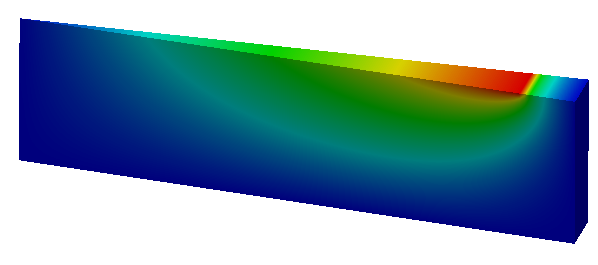
\includegraphics[width=.6\textwidth]{figures/plattenRheometerSchnitz.png}
\end{figure}
%
\subsection{Parameterfit}
Die in Kapitel \ref{Kapitel:Korrektursimulation} beschriebene Wahl der Parameter ist ein nichtlineares Ausgleichsproblem. Dabei soll die Gleichung \eqref{eq:modHB} möglichst gut an Mess- und Simulationsdaten gefittet werden, indem die Parameter $\tau_0$, $K$ und $n$ variiert werden.

Für die Lösung dieses Ausgleichproblemes wurde die Programmiersprache Python verwendet. Die Tatsache dass sie, ebenso wie \openfoam{}, frei verfügbar \todo{Lizenz abklaeren} ist und dass es unzählige schon implementierte numerische Algorithmen gibt machen Python zur idealen Wahl dafür.

Die Optimierung wurde als Python Modul \codeemph{MaT\_Optimizer} implementiert. Dabei wurde auf die Bibliotheken \codeemph{Numpy} und \codeemph{Scipy} \todo{referenz} zurückgegriffen um verschiedene Standardfunktionen zur Verfügung zu haben.\\
Das Ausgleichsproblem wird dabei mittels der Funktion \codeemph{leastsq} aus dem Modul \codeemph{optimize} von \codeemph{Scipy} gelöst.
Diese Funktion ist eine Implementierung des Levenberg-Marquardt Algorithmus, der das Problem auf eine iterative Weise löst.\\
Dazu wird eine eine enge Kopplung von Python und \openfoam{} nötig, da die Auswertung der Funktion, an die gefittet werden soll, eine Reihe von Simulationen ist.

Diese Kopplung wurde dabei mit Hilfe von \codeemph{PyFoam} \todo{Referenz} realisiert. \codeemph{PyFoam} ist eine Python Bibliothek die es ermöglicht, die von \openfoam{} als Ein- und Ausgabe benutzten Textdateien auf eine einfache Art und Weise zu erzeugen, zu ändern und auszulesen.

Um den Prozess der Parameter-Optimierung zu beschleunigen, wurde ausserdem die Bibliothek \codeemph{Parallel Python} \todo{Referenz} verwendet. Da eine Funktionsauswertung eine ganze Reihe Simulationen beinhaltet, wird dazu viel Zeit benötigt. Diese Simulationen sind aber unabhängig voneinander und können deshalb sehr einfach parallelisiert werden. Mit \codeemph{Parallel Python} können beliebig viele Prozessoren für den Parameterfit verwendet werden.

Die gemessenen Daten des Kapillarrheometers werden bereits bei der Messung durch die Verwendung des Bagley-Druckes korrigiert. Hier muss also keine Korrektursimulation durchgefue;hrt werden, die Daten koe;nnen direkt fue;r die Optimierung verwendet werden. Dies wird im Python Code berue;cksichtigt indem der Unterschied zwischen gemessenen und aus den Modell-Parametern berechneten Druckunterschiede direkt an die Fehlerfunktion angehae;ngt wird.

Ein Beispiel fue;r den Aufruf der Hauptfunktion \codeemph{runLeastSq}:
\begin{lstlisting}[language=Python]
plsq = runLeastSq(
      initialParam,            % Anfangssch@ä@tzer
      plateRheoTorque,         % Messdaten
      plateRheoOmega,          % Messdaten
      referenceCaseName,       % @\openfoam{}@ Case
      numberOfCpus,            % Anzahl Prozessoren
      kapRheoPressure,         % optionale Messdaten
      kapRheoShearRate         % optionale Messdaten
      ):  
\end{lstlisting}
%
Die genaue Dokumentation des Moduls kann in Anhang (x) \todo{Anhang schreiben} gefunden werden.
%
%\begin{lstlisting}[language=Python]
%plsq,res = leastsq(errFunc, initialParam, args=argList, maxfev=100)
%\end{lstlisting}
\subsection{Ergebnisse}
Die Anpassung der Parameter an gegebene Messdaten geschieht dank der Verwendung des \codeemph{MaT\_Optimizer} Moduls komplett automatisch. 
Die benoe;tigte Zeit hae;ngt stark von der Anzahl verwendeter Prozessoren und dem Anfangsschae;tzer ab.
%
\subsubsection{Verifikation}
Zur Verifikation des Verfahrens wurde einerseits die Qualitae;t des Parameterfits anhand der vorgegebenen Messdaten beurteilt und andererseits die resultierenden Parameter fue;r schon vermessene Moe;rtel mit alten Resultaten verglichen.

Der Vergleich mit alten Daten zeigt eine gute Übereinstimmung, die schon berechneten Parameter konnten mit einer Genauigkeit von unter x\% \todo{Uebereinstimmung angeben} nachgebildet werden.

Die Qualitae;t des Fits kann anhand des von der Funktion \codeemph{leastsq} angegebenen Residuums abgeschae;tzt werden. Dabei zeigt sich, dass das verwendete Herschel-Bulkley Modell nicht fue;r alle von Hilti eingesetzten Moe;rtel gleich gut geeignet ist. Wae;hrend fue;r die \hit{} Reihe durchwegs kleine Residuuen \todo{Zahlen} erreicht wurden, konnte der Algorithmus fue;r Moe;rtel des \re{} Typs keine gute Ue;bereinstimmung gefunden werden.\\
Dies liegt daran, dass das Herschel-Bulkley Modell die Eigenschaften des Moe;rtels nur entweder im Bereich kleiner Scherraten \todo{Zahlen} oder im Bereich von Scherraten ue;ber x\todo{Zahlen} nachbilden kann. Passende Parameter ue;ber den ganzen Bereich gibt es nicht.
%
\subsubsection{Netze}
Da die Rechenzeit einer einzelnen Simulation durch die grosse Anzahl an Simulationen sehr stark ins Gewicht fae;llt, wurde versucht ein so grobes Netz wie moe;glich zu verwenden. Natue;rlich wird dadurch der Diskretisierungsfehler immer groe;sser, weshalb ein Mittelmass zwischen benoe;tigter Simulationszeit und gemachtem Fehler gefunden werden muss.

Dazu wurde das resultierende Drehmoment bei der Verwendung verschiedener Netze verglichen. Simuliert wurde das Platte-Platte Rheometer mit Ring, mit einer no-slip Randbedingung an der unteren Wand und am Ring, einer konstanten Drehgeschwindigkeit von 10 rad/s und einem offenen Spalt zwischen oberer Platte und dem Ring.

Das verwendete Netz, dargestellt in Abbildung \ref{fig:PlattenRheoGitter:subA} ist ein hexaedrisches Gitter mit einer Zelle in tangentialer Richtung und einer Diskretisierungslae;nge von $2^{-h} \cdot 0.2\mbox{mm}$, wobei $h\in\left\{ 0,1,2,3,4 \right\}$.
%
\begin{figure}
    \centering
    \subfloat[Quadratisches Netz]{
    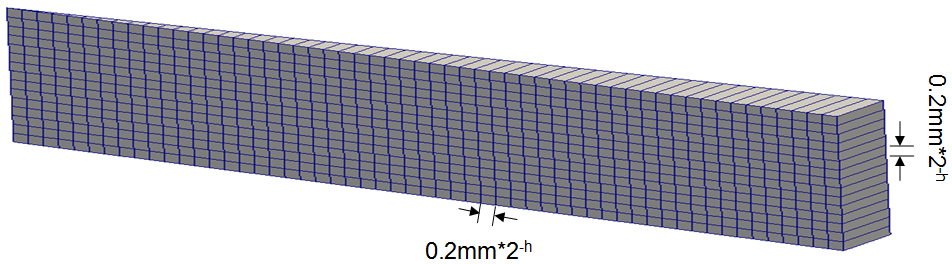
\includegraphics[width=\textwidth]{figures/PlatteRheoGitterAnnot.png}
    \label{fig:PlatteRheoGitter:subA}
    }\\
    \subfloat[O-Netz]{
    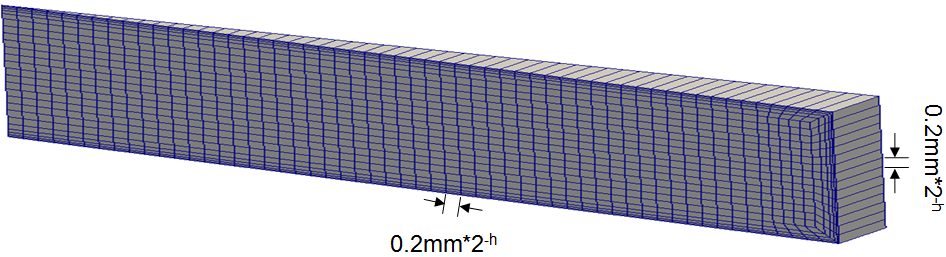
\includegraphics[width=\textwidth]{figures/PlatteRheoOGitterAnnot.png}
    \label{fig:PlatteRheoGitter:subB}
    }
    \caption{Die verwendeten Gitter fue;r die Simulation des Platte-Platte Rheometers. \subref{fig:PlatteRheoGitter:subA} ist das quadratische Netz, \subref{fig:PlatteRheoGitter:subB} das O-Netz.
    Der Parameter $h$ wurde variiert zwischen 0 und 4.}
    \label{fig:PlattenRheoGitter}
\end{figure}
%

Ebenfalls untersucht wurde das Verhalten des Drehmoments bei einer Verfeinerung der Netz-Randschicht. Dazu wurde ein O-Netz verwendet, dessen Randschicht verfeinert wurde, wie in Abbildung (x)\todo{Bild Randschicht}

Die resultierenden Werte fue;r das Drehmoment sind in Tabelle \ref{fig:ResultingTorque} aufgefue;hrt. Aufgrund der hohen Rechenzeit fue;r feinere Aufloe;sungen wurde entschieden, die Simulationen mit dem Netz $h=1$ durchzufue;hren.
%
\begin{figure}
    \centering
    \begin{tabular}{r r r r r r}
        \textbf{h} \vline & 0 & 1 & 2 & 3 & 4\\
        \hline
        \textbf{Quadr. Netz} \vline & 1.4178e-3 & 1.4353e-3 & 1.4443e-3 & 1.4479e-3 & ?.????e-3\\
        \textbf{O-Netz} \vline & 1.4381e-3 & 1.4531e-3 & 1.4514e-3 & 1.4377e-3 & ?.????e-3
    \end{tabular}
    \caption{Resultierendes Drehmoment fue;r verschiedene Netzaufloe;sungen.\\
    In der ersten Zeile ist der die Aufloe;sung bestimmende Parameter h aufgefue;hrt, in der zweiten und dritten Zeile das resultierende Drehmoment fue;r das quadratische und das O-Netz.}
    \label{fig:ResultingTorque}
\end{figure}
\todo{endgueltige Werte}
%
\subsubsection{Resultierende Parameter}
Die in dieser Arbeit untersuchten Moe;rtel tragen die Bezeichnung \hit{} und \re{}, wobei bei beiden jeweils eine A und eine B Komponente existiert (Vergleiche Kapitel \ref{Kapitel:Auspressgeraet}).\\
In Tabelle \ref{fig:resultParameter} ist eine Übersicht ue;ber die angepassten Materialparameter dargestellt, in Abbildung \ref{fig:shearVisco} sind die Messwerte und der Fit in einem doppelt logarithmischen Plot der Viskositae;t abhae;ngig von der Scherrate dargestellt.

Dabei schoe;n zu sehen ist der Einfluss des Rings, der dazu fue;hrt dass die Viskositae;tskurve beim Platte-Platte Rheometer deutlich unter den Messpunkten durchlae;uft.
Hier wurde die Viskositae;tsmessung durch den Ring verfae;lscht, was bei der Simulation wieder korrigiert wurde.
\begin{figure}
    \centering
    \begin{tabular}{l c l l l}
        \textbf{Moe;rtel} & \textbf{Komponente} & 
        \multicolumn{1}{c}{$\tau_0$} &
        \multicolumn{1}{c}{$K$} &
        \multicolumn{1}{c}{$n$} \\
        \hline
        \hline
        \multirow{2}{*}{\hit{}} & A & 199.98& 60.90& 0.62\\ 
        & B & 238.75& 34.45& 0.52\\ 
        \hline
        \multirow{2}{*}{\re{}}  & A & 108.85& 35.22& 0.71\\ 
        & B & 134.39& 37.83& 0.62
    \end{tabular}
    \caption{Übersicht ue;ber die verwendeten Modellparameter fue;r das Herschel-Bulkley Modell}
    \label{fig:resultParameter}
\end{figure}
%
\begin{figure}
    \centering
    \subfloat[\hit{} A]{
        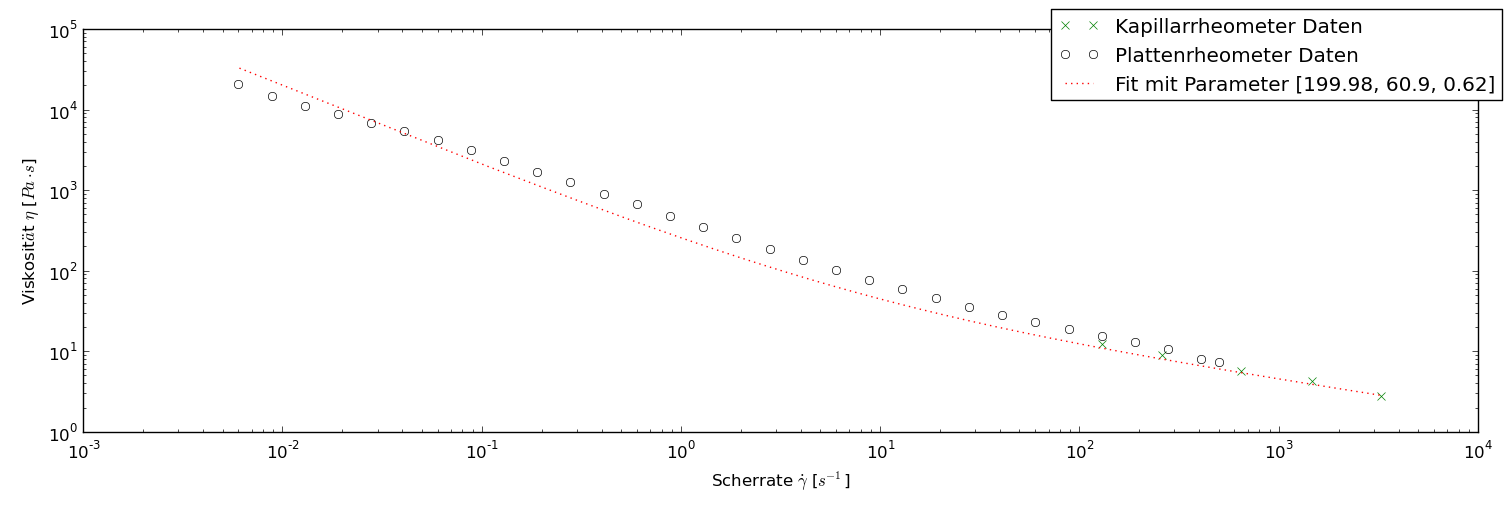
\includegraphics[width=0.47\textwidth]{figures/shearViscoMaxA.png}
        \label{fig:shearViscoHY:subA}
    }
    \subfloat[\hit{} B]{
        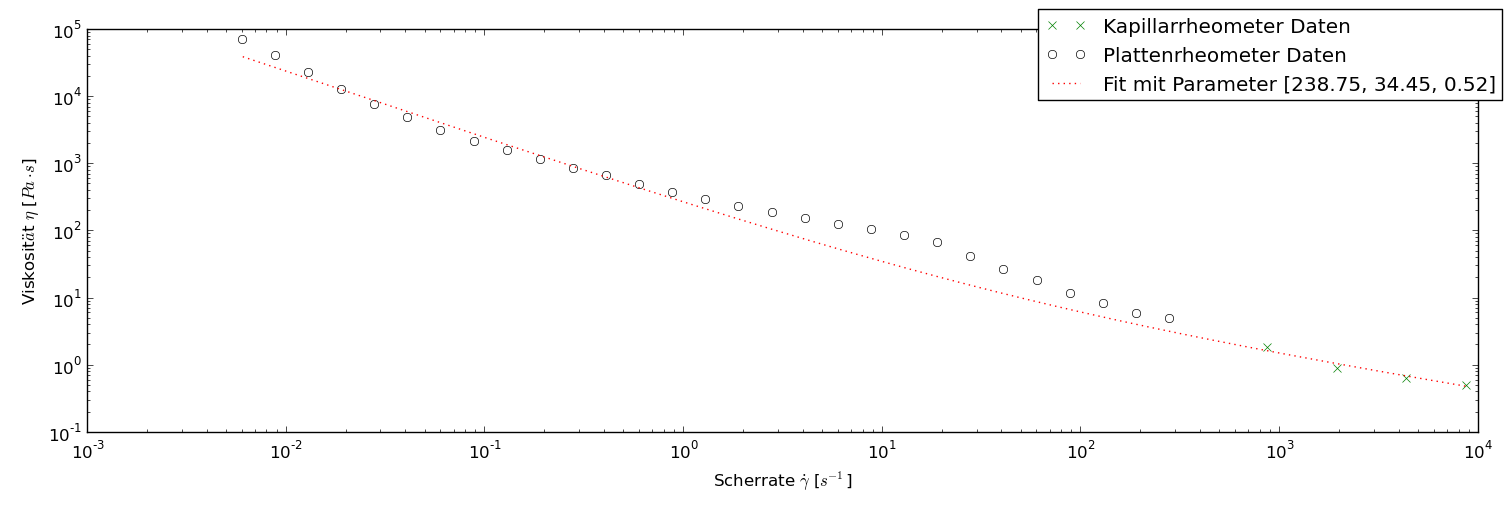
\includegraphics[width=0.47\textwidth]{figures/shearViscoMaxB.png}
        \label{fig:shearViscoHY:subB}
    } \\
    \subfloat[\re{} A]{
        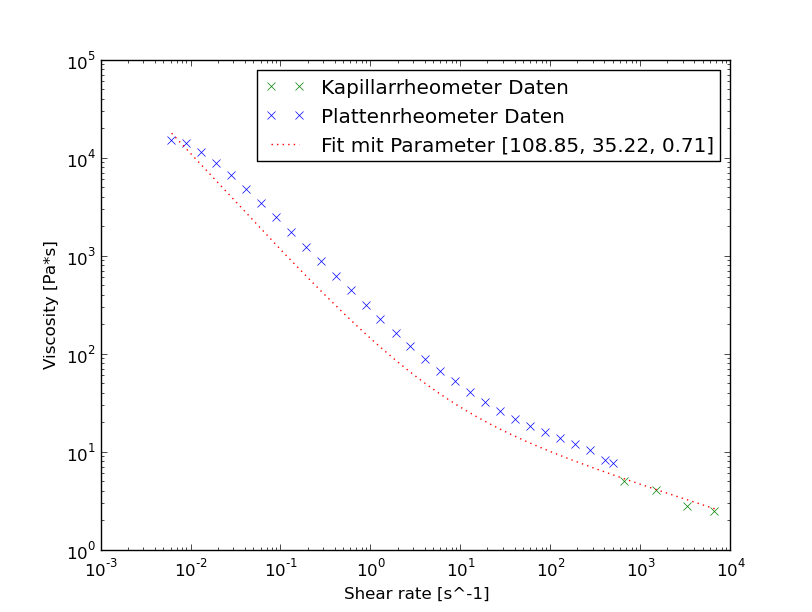
\includegraphics[width=0.47\textwidth]{figures/shearViscoReA.png}
        \label{fig:shearViscoRE:subA}
    }
    \subfloat[\re{} B]{
        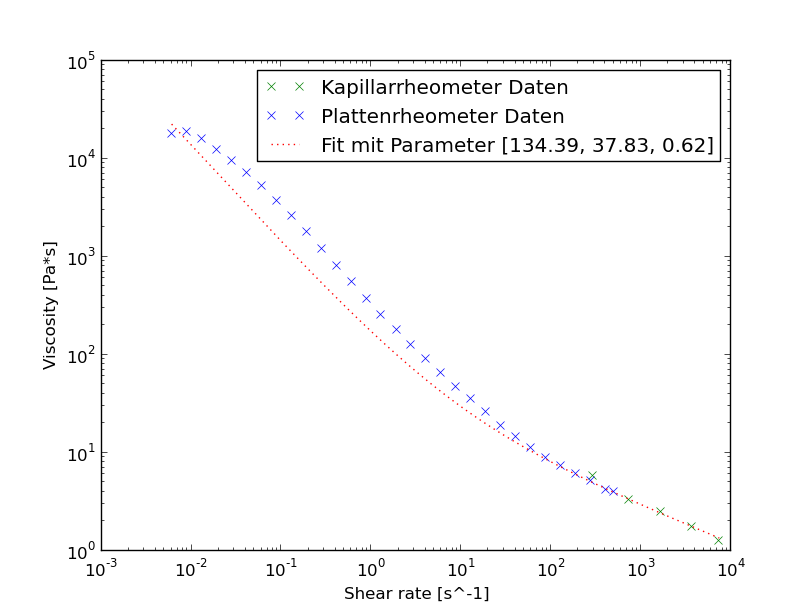
\includegraphics[width=0.47\textwidth]{figures/shearViscoReB.png}
        \label{fig:shearViscoRE:subB}
    }
    \caption{Viskositae;t abhae;ngig von der Scherrate der Moe;rtel.\\Die Kreuze sind Messpunkte aus den beiden Rheometern, die rote Kurve der daran angepasste Fit.}
    \label{fig:shearVisco}
\end{figure}
%
\subsubsection{Relaxationszeit}
Bei den Simulationen mit dem viskoelastischen White-Metzner Materialmodell \eqref{eq:whiteMetznerModell} wird zusae;tzlich zu der scherratenabhae;ngigen Viskositae;t auch ein Modell fue;r die Relaxationszeit benoe;tigt.\\
Das dazu verwendete Carreau-Yassuda Modell \eqref{eq:carreauYasuda} benoe;tigt die fue;nf Parameter $\eta_{\inf}$, $\eta_0$, $L$, $\alpha$ und $n_{\lambda}$. Da die Messung der Relaxationszeit keine Korrektursimulation benoe;tigt, kann das Modell direkt an die Messdaten gefittet werden.
Dazu wurde ebenfalls die Python-Funktion \codeemph{leastsq} verwendet. Die resultierenden Werte sind in Tabelle \ref{fig:relaxParameter} dargestellt, in Abbildung \ref{fig:shearLambda} sind die Messpunkte und der entsprechende Fit in einem Relaxationszeit - Scherraten Diagramm gezeigt.
\begin{figure}
    \centering
    \begin{tabular}{l c l l l l l}
        \textbf{Moe;rtel} & 
        \textbf{Komponente} & 
        \multicolumn{1}{c}{$\eta_{\inf}$} & 
        \multicolumn{1}{c}{$\eta_0$} &
        \multicolumn{1}{c}{$L$} & 
        \multicolumn{1}{c}{$n_{\lambda}$} & 
        \multicolumn{1}{c}{$\alpha$} \\
        \hline
        \hline
        \multirow{2}{*}{\hit{}} & A & 0.01   & 3.81  & 15.97 & 0.05 & 3       \\ 
                                & B & 0.002  & 0.18  & 40.12 & 0.65 & 1.8     \\ 
        \hline
        \multirow{2}{*}{\re{}}  & A & 0.0012 & 9.43 & 26.37  & 0.13 & 1.64    \\ 
                                & B & 0.01   & 7.8  & 70.12  & 0.04 & 2.3         
    \end{tabular}
    \caption{Übersicht ue;ber die verwendeten Modellparameter fue;r das Carreau-Yasuda Modell}
    \label{fig:relaxParameter}
\end{figure}
%
\begin{figure}
    \centering
    \subfloat[\hit{} A]{
        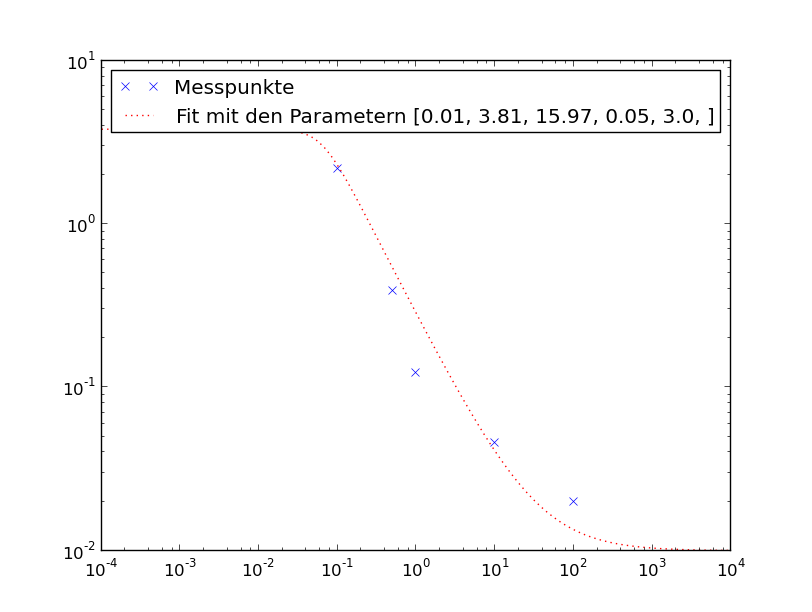
\includegraphics[width=0.47\textwidth]{figures/shearLambdaMaxA.png}
        \label{fig:shearLambdaHY:subA}
    }
    \subfloat[\hit{} B]{
        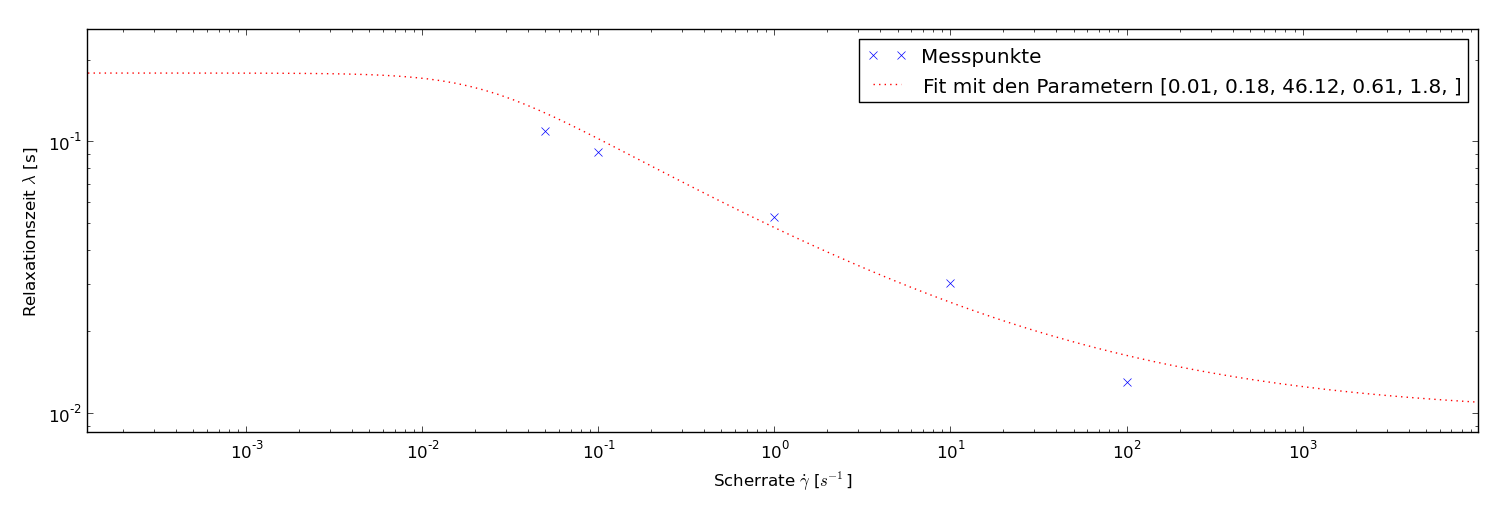
\includegraphics[width=0.47\textwidth]{figures/shearLambdaMaxB.png}
        \label{fig:shearLambdaHY:subB}
    } \\
    \subfloat[\re{} A]{
        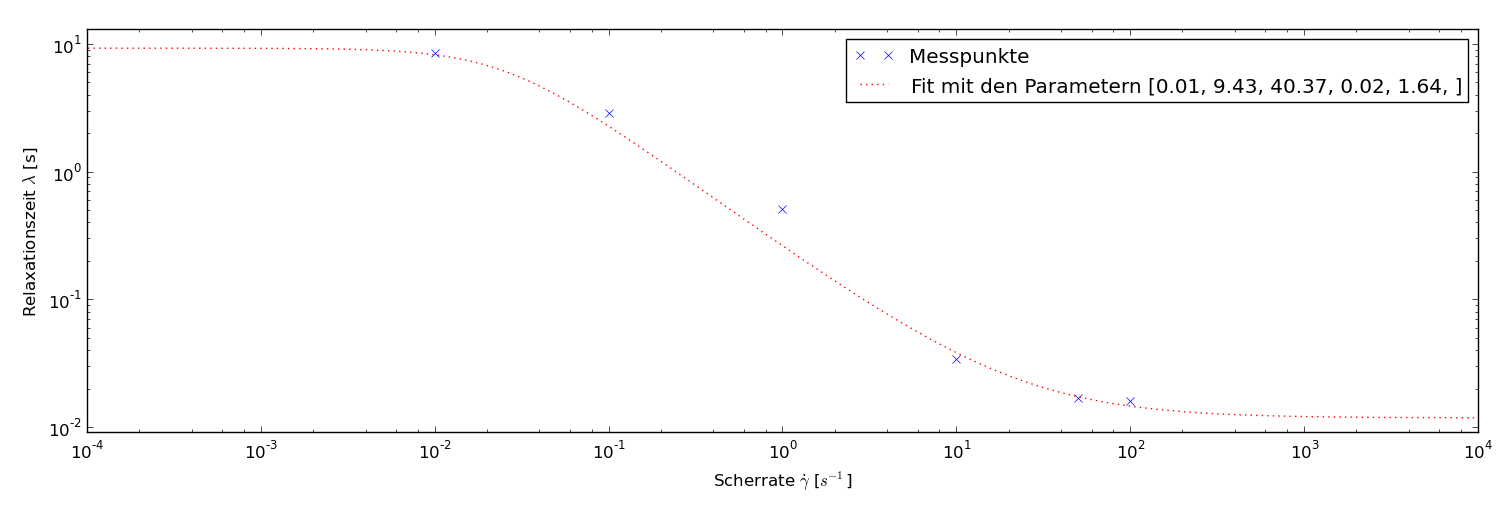
\includegraphics[width=0.47\textwidth]{figures/shearLambdaReA.png}
        \label{fig:shearLambdaRE:subA}
    }
    \subfloat[\re{} B]{
        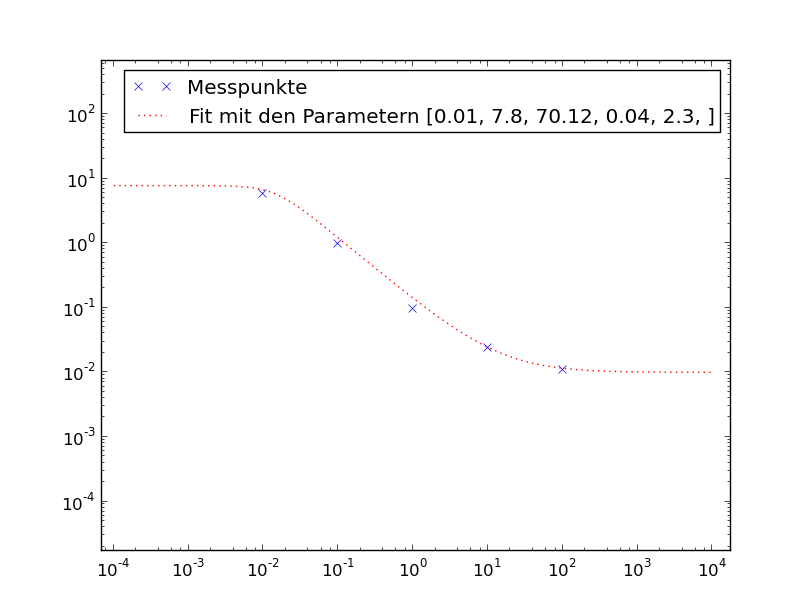
\includegraphics[width=0.47\textwidth]{figures/shearLambdaReB.png}
        \label{fig:shearLambdaRE:subB}
    }
    \caption{Relaxationszeit abhae;ngig von der Scherrate der Moe;rtel.\\Die Kreuze sind Messpunkte aus der Rheometermessung, die rote Kurve der daran angepasste Fit.}
    \label{fig:shearLambda}
\end{figure}
%
\subsubsection{Simulation Kapillarrheometer}
Das Kapillarrheometer musste fue;r die Anpassung der Parameter nicht simuliert werden. Um eine weitere Kontrollmoe;glichkeit ue;ber die Verlae;sslichkeit der Parameter zu haben wurden deshalb Simulationen des Kapillarrheometers mit Messwerten verglichen.

Zur Vermessung des Moe;rtels wurden zwei Kapillarrheometer mit verschiedenen Kapillaren verwendet. Die eine hat eine Lae;nge von $L=32\mbox{mm}$ und einen Durchmesser von $R=1\mbox{mm}$, wae;hrend die andere mit $L=16\mbox{mm}$ und $R=0.5\mbox{mm}$ nur halb so gross ist.\\
Dabei wurden sowohl Simulationen mit dem rein scherratenabhae;ngigen Modell als auch mit dem viskoelastischen Materialmodell durchgefue;hrt.

Die Simulation wurde Aufgrund der rotationssymmetrischen Geometrie ebenfalls nur fue;r einen fue;nf Grad Schnitz \todo{Ausdruck Schnitz} des Rheometers durchgefue;hrt, wie in Abbildung \ref{fig:kapRheo} \todo{Bild} zu sehen ist.\\
Das verwendete Netz wurde so skaliert, dass die Aufloe;sung nahe an der Einlassdue;se zur Kapillare sehr fein Aufgeloe;st ist, wae;hrend in Regionen die weit von der Due;se entfernt sind eine eher grobe Aufloe;sung verwendet wurde.

Zur Untersuchung des Einfluss der harten Kannte an der Einlassdue;se wurde zusae;tzlich noch ein Netz mit einer abgerundeten Kante simuliert. (Abbildung \ref{fig:roundMesh}) \todo{Einfluss Rundung} \todo{Bild}

Die Resultate sind in Tabelle \ref{fig:kapRheoResults} aufgefueh;rt.

\begin{todocontent}
    \1 Einfluss visco
\end{todocontent}
%
